\documentclass[twoside]{report}

\usepackage{geometry}
    \geometry{top=1in, bottom=1in, left=1in, right=1in}
\usepackage[utf8]{inputenc}
\usepackage[affil-it]{authblk}
\usepackage{tikz}
\usepackage{pgfplots}
\usepackage{multicol}
\usepackage{amsmath}
\usepackage{amssymb}
\usepackage{graphicx}
\usepackage[italicdiff]{physics}
\usepackage[colorlinks, allcolors=purple]{hyperref}
\usepackage{tensor}
\usepackage{upgreek}
\usepackage{mhchem}
\usepackage{comment}
\usepackage{etaremune}
% \usepackage{newtxtext, newtxmath} % Turn this on for Times New Roman, if you're a weirdo who doesn't like Computer Modern
\usepackage{fancyhdr}
    \pagestyle{fancy}
    \lhead{\leftmark}
    \rhead{\thepage}
    \cfoot{}


%%% TEXT COMMANDS %%%

\newcommand\secbf[1]{\textbf{\textsf{#1}}} % for paragraph headings
\newcommand\defbf[1]{\textbf{\textsf{#1}}} % for bolded definitions in text
\newcommand\note[1]{\fbox{
    \begin{minipage}{\linewidth}
        \textsf{\textbf{Note:} #1}
    \end{minipage}
}} % for cautionings

\newcommand\authorlist{
    Joseph R. Livesey \\
    --- add authors here ---
}

\newcommand\contributorlist{}

\newcommand\courseinfo[2]{\note{
    We took this course with \textbf{#1} in \textbf{#2.} The content and structure of the syllabus may have changed in the time since, as well as the appropriate scope of exam questions.
}}

\newcommand\highlight[1]{
    \newline\newline
    \fbox{\begin{minipage}{\linewidth}
        #1
    \end{minipage}}
    \newline\newline
} % for boxing important concepts, especially equations


%%% MATH COMMANDS %%%

\newcommand\mdv[1]{\frac{D#1}{Dt}}
\newcommand\mdvn[2]{\frac{D^#2 #1}{Dt^#2}}

\def\lsun{{L_\odot}}
\def\msun{{M_\odot}}
\def\mearth{{M_\oplus}}
\def\rsun{{R_\odot}}
\def\rearth{{R_\oplus}}
\def\HI{\textsc{Hi}}
\def\HII{\textsc{Hii}}
\def\Ha{H$\alpha$}

\DeclareMathOperator\arctanh{arctanh}
\DeclareMathOperator\arcsinh{arcsinh}
\DeclareMathOperator\arccosh{arccosh}


%%% CONTENTS %%%

\numberwithin{equation}{chapter}

\title{Astronomy Preliminary Exam \\ Study Guide}
\author{\authorlist}
\affil{University of Wisconsin--Madison}
\date{\today}

\begin{document}

\maketitle

\chapter*{Preface}

This document was created in preparation for the prelim exam in 2025, and was a collaborative effort among the students taking it that year.

The goal of this document is to provide a compact summary of the most important concepts from each of the core graduate-level astronomy courses at UW--Madison. It does not contain exam prep materials like practice problems. Nor is it an exhaustive list of the subject matter that is ``fair game'' for the prelim. It is simply meant to be used as a sort of map for studying.

This document is not meant to be read passively. Syllabi for the core astronomy courses change on an annual basis, and the original authors of this document cannot account for what new material has been cut out of or introduced to these courses since we took them. It therefore falls to the reader to be mindful of the differences between the content herein described and that covered in their own classes.

\tableofcontents

\chapter{General Knowledge}


\section{Astronomical Constants}
The following table contains constants useful for the exam. These will be useful for problems involving direct calculation, but especially for those involving order-of-magnitude estimation. The constants are given here in \defbf{CGS} (centimeter-gram-second) units and \defbf{MKS} (meter-kilogram-second) units.

Despite the fact that the reader has very likely only used MKS units before graduate school, CGS is still preferred by the writers of your exam. If that is no longer the case, it is best not to use this document for study; not because the exam will have substantially changed, but because there are bigger problems to worry about. Hell will have already frozen over, and great Birnam wood and high Dunsinane hill will both have come against you.

\begin{center}
    \begin{tabular}{|lccc|}
        \hline
        \textbf{Name} & \textbf{Symbol} & \textbf{CGS units} & \textbf{MKS units} \\
        \hline
        Gravitational constant & $G$ & $6.674 \times 10^{-8}$ dyn cm$^2$ g$^{-2}$ & $6.674 \times 10^{-11}$ N m$^2$ kg$^{-2}$ \\
        Boltzmann constant & $k_B$ & & \\
        Planck constant & $h$ & & \\
        Stefan--Boltzmann constant & $\sigma$ & & \\
        Solar luminosity & $\lsun$ & $3.828 \times 10^{33}$ erg s$^{-1}$ & $3.828 \times 10^{26}$ W \\
        Solar mass & $\msun$ & $1.988 \times 10^{33}$ g & $1.988 \times 10^{30}$ kg \\
        Electron mass & $m_e$ & $9.109 \times 10^{-28}$ g & $9.109 \times 10^{-31}$ kg \\
        Proton mass & $m_p$ & $1.673 \times 10^{-24}$ g & $1.673 \times 10^{-27}$ kg \\
        Elementary charge & $e$ & $4.803 \times 10^{-10}$ g$^{1/2}$ cm$^{3/2}$ s$^{-1}$ & $1.602 \times 10^{-19}$ C \\
        \hline
    \end{tabular}
\end{center}

If there is one thing to memorize for this exam, it is the above constants (or rather, their orders of magnitude in CGS units).


\section{Important Notation}
\subsection{Summation}
Often, particularly in Astro 702, ``Einstein notation'' is used for sums over multiple indices.\footnote{It's not actually \href{https://en.wikipedia.org/wiki/Einstein_notation}{Einstein notation}.} In this notation, an index --- say $i$ --- that is repeated within the same term implies summation over whatever set of values $i$ may take. The sum
\begin{equation}
    \sum_{i=1}^3 x_i y_i = x_1 y_1 + x_2 y_2 + x_3 y_3
\end{equation}
can thus be written
\begin{equation} \label{eq:sum-einstein}
    x_i y_i.
\end{equation}
If $x_i$ and $y_i$ denote components of vectors, then notice that (\ref{eq:sum-einstein}) amounts to a dot product, $\vb*{x} \vdot \vb*{y}$. We can also apply the repeated indices to operators, and hence we can re-write many vector operations in this notation.
\begin{align}
    \div{\vb*{u}} = \pdv{u_i}{x_i}
\end{align}

\subsection{The advective derivative}
The \defbf{advective derivative}
\begin{align} \label{eq:advective-derivative}
    \mdv{} \equiv \pdv{t} + \vb*{u} \vdot \grad{}
\end{align}
describes the time dependence of some quantity in a reference frame co-moving with a fluid parcel. In the case where there is no divergence of whatever field along a streamline ($\vb*{u} \vdot \grad{} = 0$), the advective derivative is equal to the usual (``Eulerian'') time derivative.

This operator is also known as the \textit{material, Lagrangian, Stokes, convective,} or \textit{substantive} derivative. If you write any of these on your exam, the person grading will know what you mean.

\subsection{Term symbols}
\note{It is not necessary to understand all the quantum mechanics here, only how to interpret a term symbol.} \newline

\noindent Astronomers use \defbf{term symbols} --- which are notational tools developed by atomic spectroscopists --- to uniquely identify the energy states of atoms and molecules.

Such a symbol is written for an atomic energy state as follows.
\begin{align}
    ^{2S+1}L_J
\end{align}
Here, $S$ is the total spin quantum number of the state (vector sum of all electron spins), $L$ is its total orbital angular momentum quantum number, and $J$ is its total angular momentum quantum number. These quantities satisfy the vector sum $\vb*{J} = \vb*{L} + \vb*{S}$. While we use numbers for $S$ and $J$ in a term symbol, a letter is used for $L$. The scheme for assigning these letters probably made sense to someone at some point. The first few letters are given below.
\begin{center}
    \begin{tabular}{|c|cccccc|}
        \hline
        $L$ & 0 & 1 & 2 & 3 & 4 & 5 \\
        \hline
        Designation & S & P & D & F & G & H \\
        \hline
    \end{tabular}
\end{center}
As as example, consider the ground state of carbon. Using Pauli's exclusion principle to tally up electron spins, we find that $S = 1$ (the two electrons in the outer $p$ shell contribute, each with spin $+1/2$). By similar logic, $L = 1$. In the lowest energy state, $\vb*{L}$ and $\vb*{S}$ are antiparallel, so $J = 0$.\footnote{It is extremely unlikely that a prelim question will require the derivation of a term symbol.} Hence the term symbol for the ground state of carbon is $^3$P$_0$.

While often not required, the parity of an energy state can be expressed in a term symbol. The parity is $(-1)^{\sum_i \ell_i}$, where $\ell_i$ is the orbital quantum number of each electron. An atom with parity 1 (even) can be marked with a subscript ``g'' and an atom with parity $-1$ (odd) can be marked with a subscript ``u.''\footnote{From, respectively, the German words \textit{gerade} and \textit{ungerade}.} In the ground state of carbon, it so happens that $\sum_i \ell_i = 2$, and thus the state has even parity. Its term symbol may therefore be written $^3$P$_{0,\text{g}}$.

Molecular energy states are represented somewhat differently, since unlike atoms molecules are not in general spherically symmetric. $L$ and $J$ cease to be good (meaning time-independent) quantum numbers. For a homonuclear diatomic molecule (\ce{H2}, \ce{N2}, etc.), we can take advantage of its rotational symmetry about the internuclear axis and get some new good quantum numbers. The term symbol for a molecular energy state is written in the following way.
\begin{align}
    ^{2S+1}\Lambda_\Omega%^\pm
\end{align}
It reads similarly to an atomic term symbol; $S$ is again the total spin quantum number, $\Lambda$ is the projection of the total $\vb*{L}$ along the internuclear axis, and $\Omega$ is the projection of the total $\vb*{J}$ along the internuclear axis.
% Could talk about parity again but I don't think we need to.
Once again, the orbital quantum number is denoted with a letter.
\begin{center}
    \begin{tabular}{|c|cccccc|}
        \hline
        $\Lambda$ & 0 & 1 & 2 & 3 & 4 & 5 \\
        \hline
        Designation & $\Sigma$ & $\Pi$ & $\Delta$ & $\Phi$ & $\Gamma$ & H \\
        \hline
    \end{tabular}
\end{center}

\subsection{Term diagrams}
Term diagrams show the transitions between energy levels that are possible for an atom or molecule. The ability to write out and interpret term diagrams is important for both Astro 700 and ISM.


\section{Cosmic Cliff's Notes}
What follows is a brief description of some useful concepts that apply to all areas of astrophysics.

\subsection{Timescales}
In the context of astrophysics, the word \defbf{timescale} is usually taken to mean an order-of-magnitude estimate for how long it will take for some monotonically time-dependent quantity to reach a particular value.

As an example, suppose a lone planet orbits a star with an orbital eccentricity $e$. Over time, tides raised on the planet by the star act to circularize its orbit, at a rate that is initially $\dot{e}$. We want to know roughly how long it will take for the planet to reach a circular orbit, with $e = 0$. The circularization timescale for the planet is
\begin{align}
    t_\text{circ} \sim e / \dot{e}.
\end{align}
Despite the fact that $\dot{e}$ changes non-trivially with $e$, it is acceptable to use just the initial values of $e$ and $\dot{e}$ in our estimation.\footnote{In fact, it's necessary; strictly speaking $e$ will only asymptotically approach zero. That is, if we were to do a proper analytic calculation we would find that $t_\text{circ} = \infty$, which isn't helpful.}

\subsection{Virial equilibrium}
A cloud of material that is balanced against collapse by its internal energy is said to be \defbf{virial}. It turns out that in the context of gravity (i.e., all astrophysical scenarios) such a cloud satisfies
\begin{align} \label{eq:virial-equilibrium}
    \langle U \rangle = -2\langle K \rangle,
\end{align}
where $U$ is potential energy and $K$ the internal kinetic energy. A derivation of (\ref{eq:virial-equilibrium}) is given in Appendix \ref{sec:derivation-virial-theorem}. A cloud that is in virial equilibrium is also in hydrostatic equilibrium: the state in which the outward pressure gradient force cancels the inward force of gravity. The equation of hydrostatic equilibrium is derived in Appendix \ref{sec:derivation-hydrostatic-balance}.

A virialized gas will collapse under gravity when its mass exceeds the \defbf{Jeans mass} $M_J$, or when its diameter shrinks below the \defbf{Jeans length} $\lambda_J$.


\part{Astrophysical Theory \& Methods}

\chapter{Radiation (700)}

\courseinfo{Prof. Ellen Zweibel}{Fall 2023}


\section{Radiative Transfer} \label{sec:radiative-transfer}
\subsection{The source function}
Much of astronomical science depends upon our ability to interpret light that has passed through and been modified by various media in space. In particular, continuous media both absorb incident light and emit new light. Depending on its microscopic properties, a material's capacity to absorb is parameterized by its \defbf{absorption coefficient} $\alpha_\nu$ and its production of light by its \defbf{emission coefficient} (per unit volume) $j_\nu$; these are both functions of frequency.

The relationship between these coefficients gives us the \defbf{source function}:
\begin{align} \label{eq:source-function}
    S_\nu \equiv \frac{j_\nu}{\alpha_\nu}.
\end{align}
Between two media bathed in the same radiation field at frequency $\nu$, the medium with the greater $S_\nu$ will appear brighter to an observer.

\subsection{The radiative transfer equation and its moments}
Consider light that is passing through some slab of material, perhaps a cloud in the ISM or a layer of Earth's atmosphere, with finite width. The \defbf{radiative transfer equation (RTE)} is
\begin{align} \label{eq:rte-differential}
    \dv{I_\nu}{s} = -\alpha_\nu I_\nu + j_\nu,
\end{align}
where the \defbf{optical depth} $\tau_\nu$ is defined as
\begin{equation} \label{eq:optical-depth}
    \tau_\nu(s_0, s) \equiv \int_{s_0}^s \alpha_\nu(s') \: ds'.
\end{equation}
$s - s_0$ is the path length along which light has traveled. Using the definition of the source function, we can express (\ref{eq:rte-differential}) in terms of optical depth: $\dv*{I_\nu}{\tau_\nu} = -I_\nu + S_\nu$. In integral form, we can write the RTE as
\highlight{
    \begin{equation} \label{eq:rte}
        I_\nu(s) = I_\nu(s_0) e^{-\tau_\nu(s_0, s)} + \int_{s_0}^s j_\nu(s') e^{-\tau_\nu(s', s)} \: ds'.
    \end{equation}
}
The first term on the right-hand side tells us how much of the incident light is absorbed in this slab; it starts at intensity $I_\nu(s_0)$ and then falls off exponentially as it passes through the medium. The second term tells us how much new light is emitted by the slab. The exponential under the integral sign here accounts for the fact that this new light is also getting absorbed.

\subsection{Einstein coefficients and the Einstein relations}
Consider a gas of identical atoms with two energy levels. A density $n_1$ are in the lower state, and $n_2$ in the upper state. The energy of the $1 \to 2$ transition is $h\nu_0$, and the gas receives radiation with mean intensity $J_\nu$. The rate at which atoms initially in the lower state gain energy is\footnote{Strictly speaking, we should replace $J_\nu(\nu_0)$ here with $\int d\nu \: \phi_\nu J_\nu$, where $\phi_\nu$ is the absorption line profile. However, it's okay to approximate the line profile as a delta function centered on $\nu_0$, so that $\int d\nu \: \phi_\nu J_\nu = J_\nu(\nu_0)$.}
\begin{align} \label{eq:B12}
    \left ( \pdv{n_2}{t} \right )_\text{abs} = n_1 B_{12} J_\nu(\nu_0).
\end{align}

While absorption only occurs one way, there are two ways for an atom to emit radiation: by stimulation or spontaneously. In stimulated emission, the release of a photon is caused by a resonant interaction with a photon of frequency $\nu_0$. By the same reasoning as before,
\begin{align} \label{eq:B21}
    \left ( \pdv{n_2}{t} \right )_\text{stim} = -n_2 B_{21} J_\nu(\nu_0).
\end{align}
Spontaneous emission, on the other hand, is a probabilistic phenomenon where --- undisturbed by its environment --- an atom undergoes the $2 \to 1$ transition and emits a photon.
\begin{align} \label{eq:A21}
    \left ( \pdv{n_2}{t} \right )_\text{spont} = -n_2 A_{21}
\end{align}

The rate coefficients in the above are the \defbf{Einstein coefficients}, and they are all intrinsic properties of the atom in question. The Einstein $B$ coefficients are relevant to an atom's interaction with radiation and have units erg$^{-1}$ cm$^2$ s$^{-1}$ sr. The Einstein $A$ coefficient pertains only to spontaneous emission and has units of frequency.

We can write the absorption and emission coefficients for a medium in terms of the Einstein coefficients. The former depends on both absorption and stimulated emission, since both remove background photons of a given wavelength.
\begin{align} \label{eq:absorption-coefficient}
    \alpha_\nu = \frac{1}{I_\nu} \frac{dE}{dV \: dt \: d\nu \: d\Omega} = \frac{h \nu}{4\pi} (n_1 B_{12} - n_2 B_{21}) \phi_\nu
\end{align}
Assuming isotropic emission,
\begin{align} \label{eq:emission-coefficient}
    j_\nu = \frac{dE}{dV \: dt \: d\nu \: d\Omega} = \frac{h \nu}{4\pi} n_2 A_{21} \phi_\nu
\end{align}

That the Einstein coefficients are intrinsic properties of a given atom is useful because we can derive fundamental relationships between them. These are the \defbf{Einstein relations}:
\highlight{
    \begin{equation} \label{eq:einstein-relations}
        \frac{A_{21}}{B_{21}} = \frac{2h \nu_0^3}{c^2} \quad \text{and} \quad \frac{g_1 B_{12}}{g_2 B_{21}} = 1.
    \end{equation}
}
One can obtain these equations from the assumptions of thermal equilibrium [i.e., the sum of (\ref{eq:B12}--\ref{eq:A21}) is zero and $J_\nu$ is the Planck spectrum] and infinite optical depth. Equilibrium is discussed in the next section. Note that while these assumptions make it easy to obtain the Einstein relations, they are valid even when atoms are not in thermal equilibrium.


\section{Local Thermodynamic Equilibrium}
\subsection{Temperature and the Maxwell--Boltzmann distribution}
An entity that is in \defbf{thermodynamic equilibrium} (TE) emits energy at the same rate that it receives energy. Its internal energy is constant with time. An asteroid in the Solar System, for example, is constantly heated on one side by the Sun, receiving a luminous flux of $A \lsun/4\pi r^2$, where $A$ is the surface area receiving radiation and $r$ is the Sun--asteroid distance. Therefore, the power that the asteroid radiates away must be equal to this value. Knowing this fact and that the asteroid's thermal radiation is roughly isotropic, we can figure out how bright this asteroid ought to be in the infrared.

A gas that is in TE is described by the Maxwell--Boltzmann distribution:
\highlight{
    \begin{equation} \label{eq:maxwellian}
        f(\vb*{v}) \: d^3v = \left ( \frac{m}{2\pi k_B T} \right )^{3/2} \exp(-\frac{m v^2}{2k_B T}) \: d^3v,
    \end{equation}
}
where $m$ is the mass per particle and $T$ the temperature of the gas. This distribution describes the phase space density of the gas: how many particles are in each ``bin'' of velocity. As any other density function, it is normalized such that $\int f(\vb*{v}) \: d^3v = 1$.

On Earth it is often a good assumption that if any thermodynamic entity exists unchanged long enough for you to think about it, then it is in TE. In astrophysics, however, we often deal with large physical systems, where the timescales for thermodynamic processes are very long. TE is therefore not a good \textit{a priori} assumption. For instance, taken as a whole the ISM in the Milky Way is not in equilibrium; it contains gas in many distinct phases (see \textsection\ref{sec:ism-phases}). We can, however, assume that small volumes of such a system are in equilibrium. These volumes are said to be in \defbf{local thermodynamic equilibrium} (LTE).

Temperature characterizes a system's energy balance. Therefore, a body only \textit{has} a temperature if it is in LTE. Another consequence of LTE is that a body radiates with a spectrum entirely determined by its temperature: the Planck spectrum (further discussed below).

\subsection{The Boltzmann distribution}
In a gas with a Maxwellian velocity distribution every particle has equal kinetic energy. Satisfaction of (\ref{eq:maxwellian}), therefore, is by itself a sufficient criterion to say that a gas of point particles is in LTE. However, if we want to do something useful like think about a gas of atoms or molecules, then we have additional degrees of freedom to consider. The internal energy of an atom is given by its energy state. In a gas comprising one atomic species, let $n_i$ denote the number density of atoms in the $i$-th energy state (it doesn't matter how we count states). Then, a further condition of LTE is that these densities are described by the Boltzmann distribution:
\highlight{
    \begin{equation} \label{eq:boltzmannian}
        \frac{n_j}{n_i} = \frac{g_j}{g_i} \exp(-\frac{E_j - E_i}{k_B T}).
    \end{equation}
}
This relationship applies to every pair of energy states. The factor $g_i$ is the \defbf{degeneracy} of the $i$-th state: the number of possible ways an atom can have energy $E_i$. Between two states of comparable energy, the one with greater degeneracy can host more atoms in equilibrium because it ``has more room.'' An entity with this distribution is often referred to as \textit{thermal}.

\subsection{The Saha equation}
Satisfaction of (\ref{eq:maxwellian}) and (\ref{eq:boltzmannian}) is sufficient to say that a single-species gas of neutral atoms is in LTE. But, we often have to deal with gases that contain ionized atoms and free electrons. We thus have one more condition for LTE --- the Saha equation --- that relates ionization states:
\highlight{
    \begin{equation} \label{eq:saha}
        \frac{n_{Z+1} n_e}{n_Z} = \frac{g_{Z+1} g_e}{g_Z} \left ( \frac{2\pi m_e k_B T}{h^2} \right )^{3/2} \exp(-\frac{E_{Z+1} - E_Z}{k_B T}).
    \end{equation}
}
The ionization states are indicated by the number $Z$, which is the total charge of an atom in units of the elementary charge: $q_\text{atom} = Ze$. $E_i$ here is the $i$-th ionization energy of the atom. This relationship applies to every \textit{adjacent} pair of ionization states: e.g., neutral and singly ionized, singly and doubly ionized, and so on.


\section{Electrodynamics}
\subsection{Maxwell's equations}
One will recall from their undergraduate physics courses that the four \defbf{Maxwell's equations} describe the relationship between electric field, magnetic field, charge, and current. They are presented below in CGS units, which in this case actually make things easier.\footnote{In the CGS system charge does not have a base unit; it instead derives from units of length, mass, and time. The conversion is designed such that $\varepsilon_0 = \mu_0 = 1$.}
\highlight{
    \begin{alignat}{3}
        \defbf{Gauss' law} \quad && \div{\vb*{E}} &= 4\pi \rho \\
        \defbf{Solenoidal condition} \quad && \div{\vb*{B}} &= 0 \\
        \defbf{Faraday's law} \quad && \curl{\vb*{E}} + \frac{1}{c} \pdv{\vb*{B}}{t} &= 0 \\
        \defbf{Ampère's law} \quad && \curl{\vb*{B}} - \frac{1}{c} \pdv{\vb*{E}}{t} &= \frac{4\pi}{c} \vb*{j} \\
        \nonumber
    \end{alignat}
}
Gauss' law states that a charge is a source/sink of the electric field. The solenoidal condition is that the magnetic field has no sources or sinks; there are no magnetic monopoles. Faraday's law tells us that an electric field with nonzero curl implies a changing magnetic field. Ampère's law states that a magnetic field with nonzero curl implies either a changing electric field, a nonzero current density in the direction of the curl, or both.

Note that satisfaction of the solenoidal condition means that the magnetic field can always be derived from a vector potential: $\vb*{B} = \curl{\vb*{A}}$. Let $\phi$ denote the electrostatic potential, and recall that $\vb*{E} = -\grad{\phi}$ in the absence of a magnetic field. In general we can write the electric field as
\begin{align}
    \vb*{E} = -\grad{\phi} - \frac{1}{c} \pdv{\vb*{A}}{t},
\end{align}
which we can see by taking the curl satisfies Faraday's law.

The power density of radiation is $\vb*{j} \vdot \vb*{E}$. Combining Faraday's law and Ampère's law will give us
\begin{align}
    \vb*{j} \vdot \vb*{E} = -\pdv{u_\text{EM}}{t} - \div{\vb*{S}},
\end{align}
which is a statement of energy conservation. Here
\begin{align}
    u_\text{EM} = \frac{E^2 + B^2}{8\pi}
\end{align}
is the electromagnetic energy density and
\begin{align} \label{eq:poynting}
    \vb*{S} = \frac{c}{4\pi} \vb*{E} \cp \vb*{B}
\end{align}
is the \defbf{Poynting vector}, which is in essence the electromagnetic energy flux. It therefore points out the direction in which light travels, and scales with the intensity of that light.

In vacuum, $\vb*{j} = 0$ and $\rho = 0$. Considering Maxwell's equations under these conditions, we realize we can write them in terms of the electrostatic and vector potentials. Indeed, they can be expressed as just one equation:
\begin{align} \label{eq:maxwell-vacuum}
    \laplacian{\begin{pmatrix} \phi \\ \vb*{A} \end{pmatrix}} = \frac{1}{c^2} \pdv[2]{t} \begin{pmatrix} \phi \\ \vb*{A} \end{pmatrix}.
\end{align}
The four-vector here is sometimes called the Liénard--Wiechert potential. Notice that (\ref{eq:maxwell-vacuum}) is a wave equation. If we let $\vu*{k}$ denote the direction of wave propagation, $\vb*{E} = -\vu*{k} \cp (\curl{\vb*{A}})$. The wave equation is solved by
\begin{align}
    \vb*{E} = \vb*{E}_\omega \exp[i(\vb*{k} \vdot \vb*{x} \pm \omega t)].
\end{align}
This is the electric field of radiation propagating through empty space. The field $\vb*{E}_\omega$ is a constant for light of angular frequency $\omega$, and is set by boundary conditions.

\subsection{Lag between emission and observation}
When we observe a charge at rest, we observe the potentials $\vb*{A} = 0$ and $\phi = q/r$, where $r$ is the source--observer distance. For a moving charge, we have to account for the finite speed of light; the potentials we experience due to the charge are lagged by the time it took for its radiation to reach us.
\begin{align}
    \phi = \left ( \frac{q}{\kappa r} \right )_\text{ret}, \quad \vb*{A} = \left ( \frac{q}{\kappa r} \frac{\vb*{v}}{c} \right )_\text{ret}
\end{align}
The subscripts here indicate that all quantities are to be evaluated at the time when the radiation was emitted: $t_\text{ret} = t - r/c$. $\kappa$ is a geometric factor accounting for special relativity:
\begin{align}
    \kappa_\text{ret} \equiv 1 - \frac{\vu*{k} \vdot \vb*{v}_\text{ret}}{c} = 1 - \frac{v_\text{ret}}{c} \cos(\vartheta).
\end{align}

\subsection{Dipole radiation}

\subsection{Scattering in the classical picture of atoms}


\section{Continuum Radiation}
\subsection{Blackbody radiation}
As noted previously, any source that is in LTE will emit radiation described by the Planck spectrum. In CGS units, that spectrum is
\highlight{
    \begin{equation} \label{eq:planck}
        B_\nu(\nu, T) = \frac{2h \nu^3}{c^2} \frac{1}{\exp(h \nu/k_B T) - 1}.
    \end{equation}
}
The quantity $B_\nu$ is called the spectral radiance, and it has units erg s$^{-1}$ sr$^{-1}$ cm$^{-2}$ Hz$^{-1}$. Such a source is said to radiate as a blackbody, and there is a one-to-one relationship between the peak wavelength it emits and its temperature, given by Wien's law:
\begin{align} \label{eq:wien}
    \lambda_\text{peak} = \frac{b}{T}.
\end{align}

No real source radiates as a perfect blackbody, but we tend to treat them as such and fit their spectra to a Planck spectrum to derive temperatures (e.g., stars and black hole accretion disks). Such a temperature is called an \defbf{effective temperature}, because it is strictly speaking not the real temperature of the object but instead the temperature of a hypothetical perfect blackbody that would radiate a similar spectrum.

It is important to note that for a source in LTE,
\begin{align}
    \frac{j_\nu}{\alpha_\nu} \equiv S_\nu = B_\nu.
\end{align}
This principle is often called \defbf{Kirchhoff's law}.

\subsection{Bremsstrahlung (free-free emission)}


\subsection{Cyclotron and synchrotron radiation}


\section{Polarization of Light}
Consider light initially traveling in the $\vu*{x}$ direction that undergoes Thomson scattering and travels in the $\vu*{k}$ direction thereafter. Unscattered light is polarized orthogonally to its direction of motion; initially it is polarized in the $\vu*{y}$ and $\vu*{z}$ directions. The fraction of photons initially polarized in the $\vu*{z}$ direction is $r_e^2$ (one can derive this fact from the Larmor formula). The electric field of the outgoing light is at an angle $\pi/2 - \theta$ from $\vu*{k}$, where $\theta$ is the scattering angle. Therefore, the fraction of light that gets polarized as a result of scattering is $r_e^2 \cos^2(\theta)$, and the polarization fraction of the scattered light is
\begin{align}
    \Pi = \frac{(\dv*{\sigma}{\Omega})_\text{unchanged} - (\dv*{\sigma}{\Omega})_\text{changed}}{(\dv*{\sigma}{\Omega})_\text{unchanged} + (\dv*{\sigma}{\Omega})_\text{changed}} = \frac{1 - \cos^2(\theta)}{1 + \cos^2(\theta)}.
\end{align}

The degree and manner of polarization is described by the \defbf{Stokes parameters}.
\begin{align}
    I &= I \\
    Q &= \Pi I \cos(2\psi) \cos(2\chi) \\
    U &= \Pi I \cos(2\psi) \sin(2\chi) \\
    V &= \Pi I \sin(2\psi)
\end{align}
Here, $I$ is the intensity of the light and the angles $\psi$ and $\chi$ are the orientation and ellipticity parameters of the polarization ellipse.
\begin{figure}
    \centering
    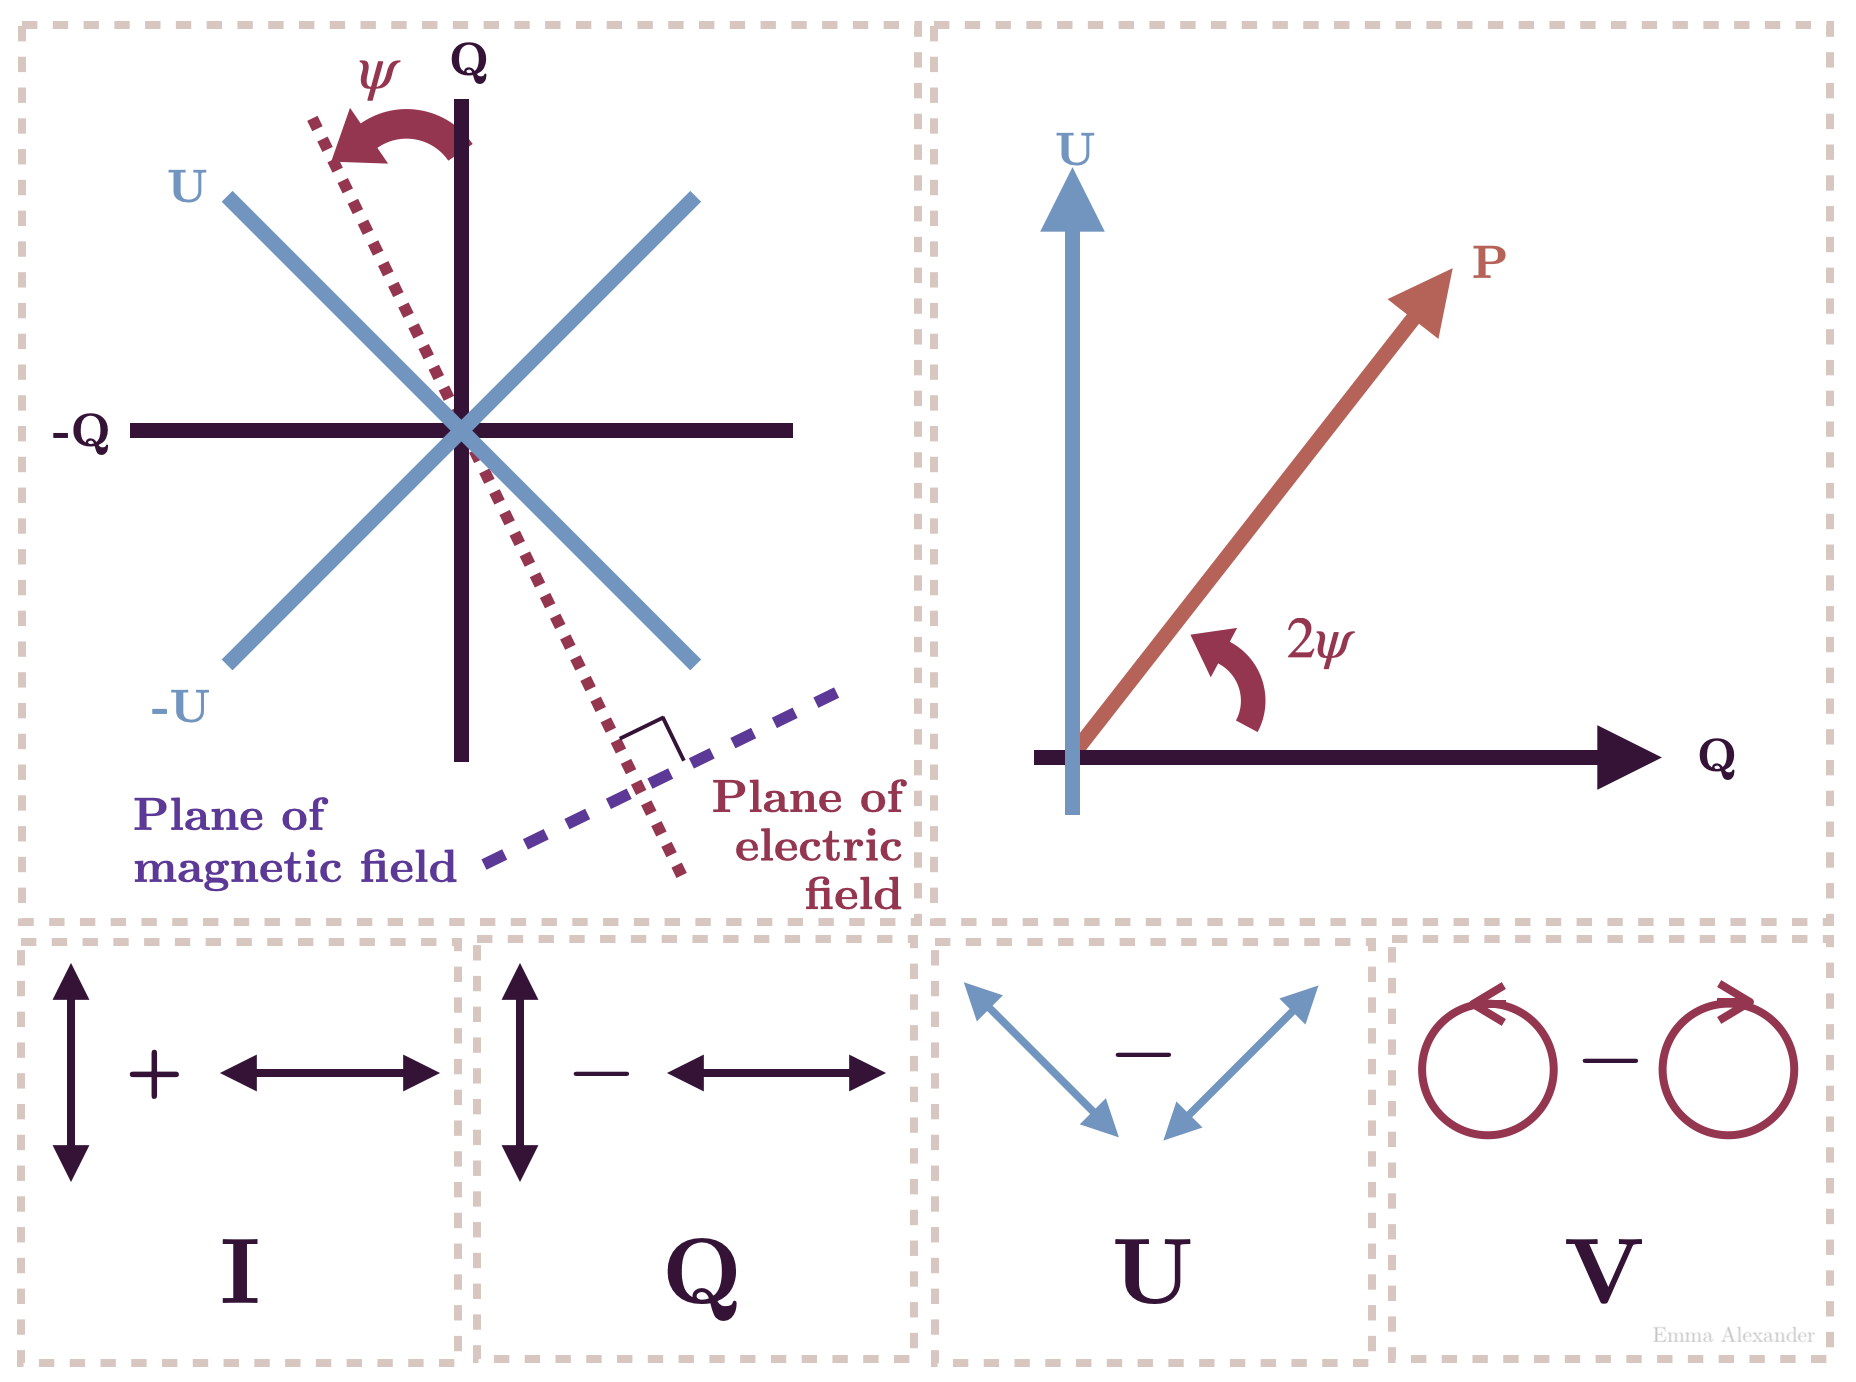
\includegraphics[width=0.5\linewidth]{figures/stokes.png}
    \caption{An illustration of the Stokes parameters. $I$ corresponds to total intensity (any direction of polarization), $Q$ gives the degree of preference for polarization along an axis, $U$ gives the degree of preference for polarization along the axis rotated $45^\circ$ from the first, and $V$ gives the degree of circular polarization.}
    \label{fig:stokes-parameters}
\end{figure}


\chapter{Dynamics (702)}

\courseinfo{Prof. Sebastian Heinz}{Spring 2024}


\section{What Is and What Is Not a Fluid?}


\section{The Fluid Equations}
\subsection{The Boltzmann equation and its moments}
We arrive at the \defbf{collisionless Boltzmann equation:}
\highlight{
    \begin{equation} \label{eq:collisionless}
        \pdv{f}{t} + \pdv{x_i} (v_i f) + \pdv{v_i} \left ( \frac{F_i}{m} f \right ) = 0.
    \end{equation}
}
If we (i) multiply through by mass $m$ and (ii) take the first moment,\footnote{Using the fact that $\int d^3v \: m \pdv*{f}{t} = \pdv*{\rho}{t}$.} we arrive at the \defbf{continuity equation:}
\begin{equation}
    \pdv{\rho}{t} + \pdv{x_i} (\rho u_i) = \pdv{\rho}{t} + \vb*{u} \vdot \grad{\rho} + \rho \div{\vb*{u}} = \mdv{\rho} + \rho \div{\vb*{u}}.
\end{equation}
\textbf{...}

\subsection{The three inviscid fluid equations}
From the collisionless Boltzmann equation we can derive the following three fluid equations (in the inviscid case).
\highlight{
    \begin{align}
        \defbf{Continuity} \quad & \pdv{\rho}{t} + \div{(\rho \vb*{u})} = 0 \label{eq:fluid-mass} \\
        \defbf{Momentum} \quad & \pdv{\vb*{u}}{t} + (\vb*{u} \vdot \grad{}) \vb*{u} = \frac{\vb*{F}}{m} - \frac{1}{\rho} \grad{P} \label{eq:fluid-momentum} \\
        \defbf{Energy} \quad & \pdv{\mathcal{E}}{t} + \vb*{u} \vdot \grad{\mathcal{E}} = -\frac{P}{\rho} \div{\vb*{u}} \label{eq:fluid-energy} \\
        \nonumber
    \end{align}
}


\section{Perfect Fluids}
\subsection{Strain}

\subsection{Barotropic flows}
In a barotropic fluid, pressure can be expressed as a pure function of density:
\begin{align}
    P = P(\rho).
\end{align}
Such a function is called an \defbf{equation of state}. Examples of barotropic fluids include:
\begin{itemize}
    \item Adiabatic ideal gases, which have the equation of state $P \propto \rho^\gamma$.
    \item Electron degenerate gases, which have the equation of state $P \propto \rho^{5/3}$.
    \item A gas in which the temperature is determined by the balance between radiative cooling and an independent heating process.
\end{itemize}
The \defbf{adiabatic index} is
\begin{align}
    \gamma \equiv \frac{C_P}{C_V} = 1 + \frac{2}{\beta},
\end{align}
where $C_P$ and $C_V$ are respectively the specific heat capacities at constant pressure and at constant volume, and $\beta$ is the number of degrees of freedom. For a (non-relativistic) ideal gas, all degrees of freedom are translational, so $\beta = 3$ and $\gamma = 5/3$.

For a barotropic, irrotational flow we can write the flow velocity as the gradient of a scalar potential, $\vb*{u} = \grad{\phi}$. This phenomenon is termed \defbf{potential flow}. If the flow is stationary (meaning $D\rho/Dt = 0$), then the continuity equation (\ref{eq:fluid-mass}) becomes simply
\begin{align}
    \laplacian{\phi} = 0,
\end{align}
which is Laplace's equation. To solve for potential flow in the presence of some obstacle, we first assume a constant background velocity $\vb*{u}_0 = u_0 \vu*{x}$, which implies the background potential $\phi_0 = u_0 x$. We identify a boundary condition at the obstacle (e.g., the component of $\vb*{u}$ normal to the surface must be zero). Then, we write out Laplace's equation in whatever co-ordinate system is most convenient and solve for $\phi$.

\subsection{The vorticity equation}
The \defbf{vorticity} of a fluid $\vb*{\omega} \equiv \curl{\vb*{u}}$ becomes nonzero when surfaces of constant density and surfaces of constant pressure are misaligned with respect to one another. Taking the curl of the momentum equation (\ref{eq:fluid-momentum}) yields the vorticity equation
\begin{align}
    \pdv{\vb*{\omega}}{t} = (\vb*{\omega} \vdot \grad) \vb*{u} - \vb*{\omega} (\div{\vb*{u}}) + \frac{1}{\rho^2} (\grad{\rho} \cp \grad{P}).
\end{align}
One can replace $\vb*{u} \to \vb*{u}_\perp$ in this equation, where $\vb*{u}_\perp$ is the component of the velocity parallel to the vorticity, since the terms containing $\vb*{u}_\parallel$ cancel. In an initially irrotational fluid, the only thing that can create vortices is a nonzero $\grad{\rho} \cp \grad{P}$; this is called the baroclinic term.

Let $\Gamma = \oint d\vb*{\ell} \vdot \vb*{u}$ denote the \defbf{circulation} of a fluid around some closed curve. Clearly in an irrotational fluid, $\Gamma = 0$ globally. Stokes' theorem allows us to re-write the circulation as $\Gamma = \int d\vb*{A} \vdot \vb*{\omega}$. Integration of the vorticity equation gives us
\begin{align}
    \dv{\Gamma}{t} = \frac{1}{\rho^2} \int d\vb*{A} \vdot (\grad{\rho} \cp \grad{P}),
\end{align}
from which we gather that for a barotropic, incompressible fluid the circulation is conserved. This idea is the Kelvin circulation theorem.

\subsection{Bernoulli's law}
Take the momentum equation (\ref{eq:fluid-momentum}) and assume a conservative force, so that the acceleration of a parcel is $\vb*{F}/m = -\grad{\Phi}$. Dotting the resulting equation with $\vb*{u}$ yields the Bernoulli equation
\begin{align} \label{eq:bernoulli}
    \mdv{} \left ( \tfrac{1}{2} u^2 + \Phi + H \right ) = 0,
\end{align}
where $H = \int dP/\rho$ is the (specific) enthalpy. The term in parentheses is the \defbf{Bernoulli constant} $\mathcal{B}$, which (\ref{eq:bernoulli}) tells us is conserved along streamlines. It is usually most easily evaluated at infinity, where $\Phi = 0$.

It is useful to note that the Bernoulli equation is really nothing more than a statement of conservation of energy. We have specific kinetic energy $\tfrac{1}{2} u^2$, potential energy $\Phi$, and internal (thermal + $P \: dV$) energy $H$, and their sum is constant.


\section{Viscous Fluids}
\subsection{The Navier--Stokes equation}

\subsection{Turbulence and the Reynolds number}


\section{Waves and Instabilities}
\subsection{Linearization of the fluid equations}
The fluid equations are nonlinear, but we can linearize them by breaking each of the three time-dependent quantities into a background value and a perturbation: $P = P_0 + P'$, $\rho = \rho_0 + \rho'$, and $\vb*{u} = \vb*{u}_0 + \vb*{u}'$. This approach is valid because changes in these quantities will always be small relative to their absolute values. Substituting these expressions into the fluid equations (\ref{eq:fluid-mass}--\ref{eq:fluid-energy}) and doing some algebra yields new equations broken into background, perturbation, and mixed terms. We drop all second-order terms (those that contain a product of two perturbations, which will be very small). Then, we assume that the background is hydrostatic, so that we can set $\vb*{u}_0 = 0$. Our PDEs are now
\begin{align}
    \pdv{\rho'}{t} + \div{(\rho_0 \vb*{u}')} &= 0 \label{eq:linear-continuity} \\
    \pdv{\vb*{u}'}{t} + \frac{1}{\rho_0} \grad{P'} - \frac{\rho'}{\rho_0^2} \grad{P_0} &= \frac{\vb*{F}'}{m} \label{eq:linear-momentum} %\\
    % P &= P_0 \left ( \frac{\rho}{\rho_0} \right )^\gamma.
\end{align}
Note that we have omitted the energy equation because we don't need it; if we know the equation of state we can substitute $P(\rho)$ into the continuity and momentum equations to obtain two linear equations in two variables: $P'$ and $\vb*{u}'$.

\subsection{Acoustic waves}
Assume the background quantities like $P_0$ are constant everywhere; their gradients are zero. Therefore, taking the divergence of the linearized momentum equation (\ref{eq:linear-momentum}) gives us
\begin{align}
    \pdv[2]{P'}{t} = \pdv{P}{\rho} \laplacian{P'},
\end{align}
which is the acoustic wave equation. Such a wave has the characteristic velocity $a_s \equiv \sqrt{\pdv*{P}{\rho}}$, which is the speed of sound in the medium. In an adiabatic ideal gas, $P = P_0 (\rho/\rho_0)^\gamma$, this is the \defbf{adiabatic sound speed} $a_s = \sqrt{\gamma P_0/\rho_0}$. In an isothermal gas $\gamma = 1$ and this speed is the \defbf{isothermal sound speed} $c_s = \sqrt{P_0/\rho_0}$.

The propagation of acoustic waves with wavevector $\vb*{k}$ is given by the \defbf{phase velocity}
\begin{align}
    \vb*{c}_p = \frac{\omega}{k^2} \vb*{k}.
\end{align}
The relationship between angular frequency and wavenumber $\omega = \omega(\vb*{k})$ for any type of wave is its \defbf{dispersion relation}. For acoustic waves, $\omega(\vb*{k}) = \pm a_s \norm{\vb*{k}}$.

\subsection{Kelvin--Helmholtz instability}

\subsection{Rayleigh--Taylor instability}


\section{Shocks}
\subsection{Normal shocks and the jump conditions}

\subsection{Oblique shocks}

\subsection{Blast waves}
In an explosion (e.g., a supernova) a large amount of thermal energy is released instantaneously within a small volume. As long as the internal pressure is much greater than the ram pressure of the surrounding ISM, then the resulting blast wave will accelerate as it expands. Such a blast wave is an instance of a strong shock.

The \defbf{Sedov--Taylor solution} approximates the radius of the resulting blast wave at a given time $t$ after an explosion. It is:
\highlight{
    \begin{equation} \label{eq:sedov-taylor}
        r_\text{shock} = \xi_0 \left ( \frac{E t^2}{\rho_\text{ISM}} \right )^{1/5}.
    \end{equation}
}
While a somewhat crude approximation, this equation is extremely useful because it is (i) simple and (ii) only requires that we know the energy of the explosion and the density of the surrounding ISM. The Sedov--Taylor solution is derived from dimensional analysis alone. The similarity variable $\xi_0$ is dimensionless.\footnote{It is called the \textit{similarity variable} because it fully encapsulates the relationship between time and radius. Blast waves with the same $\xi_0$ evolve identically.} One will not be asked on the exam to calculate the similarity variable; it is a highly non-trivial function of the adiabatic index. $\xi_0 \sim 1$ suffices for order-of-magnitude estimation.

The Sedov--Taylor solution has some notable limitations. In particular, it assumes:
\begin{itemize}
    \item $\rho_\text{ISM}$ is constant (i.e., the ISM was not disturbed by the progenitor).
    \item The explosion was long enough ago that the mass swept up in the shock exceeds the mass of the explosion ejecta (the latter is unaccounted for).
    \item The explosion was not long enough ago that radiative cooling has significantly changed the internal pressure of the blast wave.
\end{itemize}


\section{Magnetohydrodynamics}
\subsection{The MHD equations}

\subsection{Alfvén waves}

\subsection{Fast and slow modes}



\chapter{Observational Techniques (500)}

\courseinfo{Dr. Nicholas McConnell}{Fall 2024}


\section{Tallying Light}
\subsection{Flux and surface brightness}

\subsection{Filters and magnitude systems}


\section{Detectors, Signal, and Noise}
\subsection{Detectors and detector noise}

\subsection{Noise distribution and error propagation}

\subsection{Signal-to-noise regimes}
In total, the formula for calculating S/N is
\begin{equation} \label{eq:s/n}
    \frac{S}{N} = \frac{S}{\sqrt{S + B + R + D}},
\end{equation}
where $S$ is the observed signal from the target source, $B$ is the sky signal, $R$ is the read noise, and $D$ is the dark current in the detector. Let $A$ be the detector area, $\varepsilon$ the system efficiency, $f_\text{obs}$ the flux of light from the target, $I_\text{sky}$ the sky brightness, $\Omega$ the solid angle observed, $N_R$ the intrinsic read noise of the instrument per pixel, $N_D$ the dark noise per pixel per unit time, $G$ the gain, $n$ the number of pixels in the detector, and $t$ the total time for which the observation was taken. Then, the terms in the denominator of (\ref{eq:s/n}) are
\begin{equation}
    S = A \varepsilon f_\text{obs} t, \quad B = A \varepsilon I_\text{sky} \Omega t, \quad R = \left ( N_R + \tfrac{1}{2} G \right )^2 n, \quad D = N_D n t.
\end{equation}
Sometimes one of these terms dominates over the others, and in that case the S/N is largely set by that term. For instance, observations can be sky noise-limited or read noise-limited. Note the time dependence of (\ref{eq:s/n}) in these cases; if read noise dominates then S/N $\propto t$, whereas if read noise is much smaller than the other terms then S/N $\propto \sqrt{t}$. In any case, S/N always increases with time.


\section{Optics, Telescopes, and Spectrographs}
\subsection{Telescope optics}

\subsection{Diffraction gratings and spectrographs}


\section{Planning Observations}



\part{Astrophysical Systems}

\chapter{Stellar Interiors \& Evolution (715)}

\courseinfo{Prof. Rich Townsend}{Spring 2025}

\chapter{The Interstellar Medium (720)}

\courseinfo{Prof. Susanna Widicus Weaver}{Spring 2024}


\section{The Phases of the ISM} \label{sec:ism-phases}
The ISM consists of several distinct phases. They are listed in the table below with characteristic temperatures, number densities, and the state of hydrogen within each.
\begin{center}
    \begin{tabular}{|ccccc|}
    \hline
         \textbf{Phase} & \textbf{Temperature} & \textbf{Density} & \textbf{H state} & \textbf{Observed through} \\
         & \textbf{(K)} & \textbf{(cm$^{-3}$)} & & \\
         \hline
         Molecular clouds & 10--20 & 10$^2$--10$^6$ & molecular & radio and infrared lines \\
         Cold neutral medium & 50--100 & 20--50 & neutral & \HI~21 cm absorption \\
         Warm neutral medium & 6000--10000 & 0.2--0.5 & neutral & \HI~21 cm emission \\
         Warm ionized medium & 8000 & 0.2--0.5 & ionic & \Ha~emission \\
         \HII~regions & 8000 & 10$^2$--10$^4$ & ionic & \Ha~emission \\
         Hot ionized medium & 10$^6$--10$^7$ & 10$^{-4}$--10$^{-2}$ & ionic (metals too) & X-ray emission, \\
         & & & & metal UV absorption \\
         \hline
    \end{tabular}
\end{center}
Each of these components is well mixed (read: in LTE), but is perturbed by dynamic processes like stellar winds and supernovae. The ISM is heated by the interstellar radiation field (electromagnetic) and by cosmic rays. It is permeated by magnetic fields, while gravitational fields are really only important in dense clouds.


\section{Radiative Transfer Redux} \label{sec:ism-rt}
At this point the reader is directed back to \textsection\ref{sec:radiative-transfer} for a more detailed discussion of the radiative transfer equation and the Einstein coefficients. The discussion of radiative transfer here is specific to concepts relevant to the ISM.

\subsection{Interaction of light and the ISM}

\subsection{Line shapes}


\section{Collisional Excitation} \label{sec:ism-collisional}


\section{Optical and UV Absorption Features} \label{sec:ism-absorption}
\subsection{The curve of growth}


\section{The 21 cm Line} \label{sec:ism-21cm}


\section{Molecular Clouds} \label{sec:ism-clouds}


\section{Photoionization and HII Regions} \label{sec:ism-photoionization}


\section{Dust} \label{sec:ism-dust}
Interstellar \defbf{dust} is an important component of the ISM. It plays a role in ISM chemistry, and modifies the interstellar radiation field by absorbing light and re-emitting it at thermal (infrared) wavelengths. There is ample observational evidence for dust in the Milky Way, including: (i) depletion of refractory elements from the gas-phase ISM, (ii) extinction of background starlight, (iii) infrared emission, (iv) optical polarization, and (v) relic grains found in meteorites on Earth.

Dust grains range in size from \defbf{PAH}s (polycyclic aromatic hydrocarbons; size $\sim 10$ \r{A}, density\footnote{A linear density is given along the line of sight.} $\sim 1$ cm$^{-1}$) to ``large grains'' (size $\sim 10^3$ \r{A}, density $\sim 10^{-8}$ cm$^{-1}$). PAHs are complex organic molecules with 20--50 carbon atoms that we often see through absorption lines at superpositions of their many vibrational modes.

Dust is composed of

Let $Q_\text{abs}$ denote the emissivity of a grain and $a$ its radius, and assume an isotropic radiation field $J_\lambda$. The heating rate for this dust is then
\begin{align}
    \Gamma = (4\pi \text{ sr}) \times \int_0^\infty J_\lambda Q_\text{abs} \: d\lambda \times (\pi a^2).
\end{align}
The emissivity is close to unity when the dust grain cross section is much larger than the wavelength. This is true for UV radiation, which accounts for most heating of dust. In this case $Q_\text{abs} \sim 1$ and we have
\begin{align}
    \Gamma_\text{UV} = 4\pi^2 a^2 J_\text{UV},
\end{align}
where $J_\text{UV} \simeq \int_0^\infty J_\lambda \: d\lambda$. Assuming TE we can apply Kirchhoff's law to obtain $J_\text{UV} = \sigma T_d^4 \langle Q_\text{abs} \rangle$, where $\langle Q_\text{abs} \rangle$ is the ``Planck-average'' emissivity. $T_d$, the equilibrium dust temperature, depends on the radiation field, and we can therefore use the empirically derived power law relationship
\begin{align}
    \langle Q_\text{abs} \rangle \propto a T_d^\beta,
\end{align}
where $\beta \simeq 2$. Typical dust temperatures in the diffuse ISM are $\sim 10$ K. In \HII~regions they are more like $\sim 10^2$ K (compare to gas temperature of $\sim 10^4$ K).

The \defbf{gas-to-dust ratio} tells us the relative amount of dust that is present in a column. Using the $B - V$ color excess $E(B - V) = A_\nu/R_\nu$, the gas-to-dust ratio is
\begin{align}
    \frac{M_H}{M_d} = \frac{N_H}{E(B - V)}
\end{align}
Note that $N_H$ is the column density for hydrogen \textit{atoms}; we would double-count \ce{H2}, for example. This ratio is often used as a proxy for metallicity.




\chapter{Galaxies (730)}

\courseinfo{Prof. Matt Bershady}{Fall 2023}


\section{Stellar Populations}


\section{ISM}


\section{Environment}


\section{Dynamics}


\section{Morphology}
\subsection{Spiral galaxies}

\subsection{Elliptical galaxies}

\subsection{Dwarf galaxies}


\section{Evolution}


\chapter{Observational Cosmology (735)}

\courseinfo{Prof. Michael Maseda}{Spring 2025}

\part*{Appendix}

\addcontentsline{toc}{part}{\bfseries Appendix}
\renewcommand{\chaptername}{Appendix}
% \renewcommand{\thechapter}{\Alph{chapter}}
% \setcounter{chapter}{0}
\renewcommand{\thechapter}{A} % This is a hack --- should be able to reset the counter and have lettered chapters separate from numbered chapters somehow


\chapter{Derivations}


\section{Hydrostatic Balance} \label{sec:derivation-hydrostatic-balance}
Consider a thin spherical shell of material in a body, like a star or planet, that is held in equilibrium by a balance between gravity and the pressure gradient force. Recall that pressure has units of force/area; naturally the pressure gradient force felt by this shell of fluid can be written $A \Delta P$, where $A$ is the surface area of the shell and $\Delta P$ is the difference between the pressure at the bottom and top of the layer. The gravitational force experienced by this layer, meanwhile, is $-M g$, where $M = A \Delta z \rho$ is its total mass. Setting these forces equal, the surface area cancels out:
\begin{align}
    \Delta P &= -\rho g \Delta z.
\end{align}
In the limit of an infinitesimally thin shell, we are left with the differential equation
\highlight{
    \begin{equation}
        dP = -\rho g \: dz.
    \end{equation}
}

We could also start from the vertical component of the Navier--Stokes equation. If we assume a barotropic fluid in which gravity is the only external force, the other terms disappear and we are left with
\begin{align}
    \frac{1}{\rho} \pdv{P}{z} &= \frac{F_z}{m} \\
    \pdv{P}{z} &= -\rho g.
\end{align}

In Earth's ocean we can approximate both the density and gravitational acceleration as constant, and we have a pressure that changes linearly with depth:
\begin{align}
    P \propto -\rho_0 g_0 z.
\end{align}
For the interior of a star, however, both of these assumptions are poor. The density changes with pressure according to a polytropic equation of state: $\rho(P) \propto P^{n/(n+1)}$. The gravitational acceleration at radial distance $z$ is $g = G M(z) / z^2$, where $M$ is the mass interior to $z$.


\section{The Virial Theorem} \label{sec:derivation-virial-theorem}
Consider a gravitationally bound collection of $N$ particles. The $i$-th particle has mass $m_i$, position $\vb*{r}_i$, velocity $\vb*{v}_i$, and momentum $\vb*{p}_i$. In the center-of-mass reference frame, this gas has moment of inertia
\begin{align}
    I  = \sum_{i=1}^N m_i \vb*{r}_i \vdot \vb*{r}_i.
\end{align}
Differentiation gives us
\begin{align} \label{eq:moi-derivative}
    \dv{I}{t} = 2 \sum_i m_i \vb*{v}_i \vdot \vb*{r}_i = 2 \sum_i \vb*{p}_i \vdot \vb*{r}_i.
\end{align}
Differentiating again, we have
\begin{align}
    \dv[2]{I}{t} = 2 \left ( \sum_i \dv{\vb*{p}_i}{t} \vdot \vb*{r}_i + \sum_i \vb*{p}_i \vdot \dv{\vb*{r}_i}{t} \right ) = 2 \left ( \sum_i \vb*{F}_i \vdot \vb*{r}_i + \sum_i m_i \vb*{v}_i \vdot \vb*{v}_i \right ).
\end{align}
The average of (\ref{eq:moi-derivative}) over some span of time $\tau$ is given by
\begin{align} \label{eq:moi-derivative-avg}
    \left\langle \dv{I}{t} \right\rangle = \frac{1}{\tau} \int_0^\tau \dv[2]{I}{t} \: dt.
\end{align}
For a virialized system, there will be no secular changes in the moment of inertia; $\langle dI/dt \rangle = 0$. This fact implies that the integrand in (\ref{eq:moi-derivative-avg}) is also zero, and thus
\begin{align}
    \sum_i \vb*{F}_i \vdot \vb*{r}_i = -\sum_i m_i \vb*{v}_i \vdot \vb*{v}_i.
\end{align}
The left-hand side is the combined average gravitational potential energy of all the particles, and the right-hand side is twice their combined average kinetic energy.
\highlight{
    \begin{equation} \label{eq:virial-theorem}
        \langle U \rangle = -2\langle K \rangle
    \end{equation}
}
We have arrived at the virial theorem we all know and love.


\section{The Jeans Length and the Jeans Mass}
When a gas in virial equilibrium shrinks to a scale less than its Jeans length, it will undergo gravitational collapse. That is, the gravitational potential energy of the gas must overcome its internal (kinetic) energy. Assume TE, so that we can write down the internal energy in terms of a temperature. The gravitational potential energy is
\begin{align}
    \frac{G M m}{r^2} = \tfrac{4}{3} \pi G \rho m r,
\end{align}
where $M$ is the total mass of the cloud and $m$ is the mass of each particle (or the mean molecular weight of a multi-species cloud). The internal energy, assuming a monatomic ideal gas, is
\begin{align}
    \tfrac{3}{2} N k_B T = \frac{}{}
\end{align}


\section{The Free-Fall Time}
The free-fall time is the timescale on which a spherical cloud will collapse under its own gravity, neglecting any other forces. First consider a single particle in the cloud, which begins at a distance $R$ from the center.

Kepler's third law tells us the period of any two-body orbit with semi-major axis $a$, and applies regardless of the orbit's eccentricity.
\begin{align}
    P = 2\pi \sqrt{\frac{a^3}{G M}}
\end{align}
A straight trajectory towards the center of mass is equivalent to a Keplerian orbit with $e = 1$. The semi-major axis is the average distance of an orbiting body: $a = R/2$ for this trajectory. The free-fall time will be half of the orbital period here (since the particle will go down and not back up).
\begin{align}
    t_\text{ff} = \frac{P}{2} = \pi \sqrt{\frac{(R/2)^3}{G M}}
\end{align}
In the single-particle picture, $M$ is just the mass of the body towards which the particle is falling. In the context of a collapsing cloud of many particles, we will assume a spherically symmetric cloud of uniform density, so that gravitational interactions between this particle at distance $R$ and all particles exterior to $R$ cancel out. All that matters are the particles interior to $R$; the relevant mass is
\begin{align}
    M = \tfrac{4}{3} \pi R^3 \rho,
\end{align}
where $\rho$ is the mass density interior to $R$. Thus,
\highlight{
    \begin{align}
        t_\text{ff} = \sqrt{\frac{3\pi}{32G \rho}}.
    \end{align}
}


\section{Kepler's Second Law}
Unless the exoplanets course is added to the prelim in the future, it is unlikely that Kepler's laws will be a topic of much importance to the exam. However,

Stated in words, Kepler's second law is that an orbiting body sweeps out equal areas in equal spans of time.

Recall that the angular momentum of a mass $m$ may be written $\vb*{r} \cp m \vb*{v}$. The specific angular momentum of a body on a Keplerian orbit is thus $\vb*{h} = \vb*{r} \cp \vb*{v}$, in a co-ordinate system centered on the body it orbits.
\begin{align}
    \dv{\vb*{h}}{t} = \dv{\vb*{r}}{t} \cp \vb*{v} + \vb*{r} \cp \dv{\vb*{v}}{t}
\end{align}


\end{document}